\subsection{Oberfl�che}

Der allgemeine Aufbau der \gls{gui} der \gls{bts} wurde schon im Punkt \ref{aufbauGUI} "`Aufbau der grafischen Benutzeroberfl�che"' erl�utert. Im folgenden soll allerdings zus�tzlich ein Einblick in die Darstellung erfolgreicher Berechnungen gegeben werden.\\
\\
Nachdem in der \gls{bts} ein entsprechendes Algorithmus-\gls{dll}-File und ein Daten-\gls{csv}-File ausgew�hlt wurden, k�nnen ggf. noch Einstellungen angepasst und anschlie�end die Berechnung gestartet werden. Nun wird zuerst das Daten-File eingelesen, dann werden mit dem Algorithmus Signale berechnet, und schlussendlich errechnet die \gls{bts} Performancedaten und aktualisiert die \gls{gui}. Bei unserem fertigen Regressionsalgorithmus und einem passenden Daten-File von Google �ber 300 Tage (daily-Bars) werden die allgemeinen Performancedaten bei Standardeinstellungen und einem Startkapital von \$ 100,00.00, wie in Abbildung \ref{fig:bts_performance} ersichtlich, angezeigt.\\

\begin{figure}[!h]
	\centering
		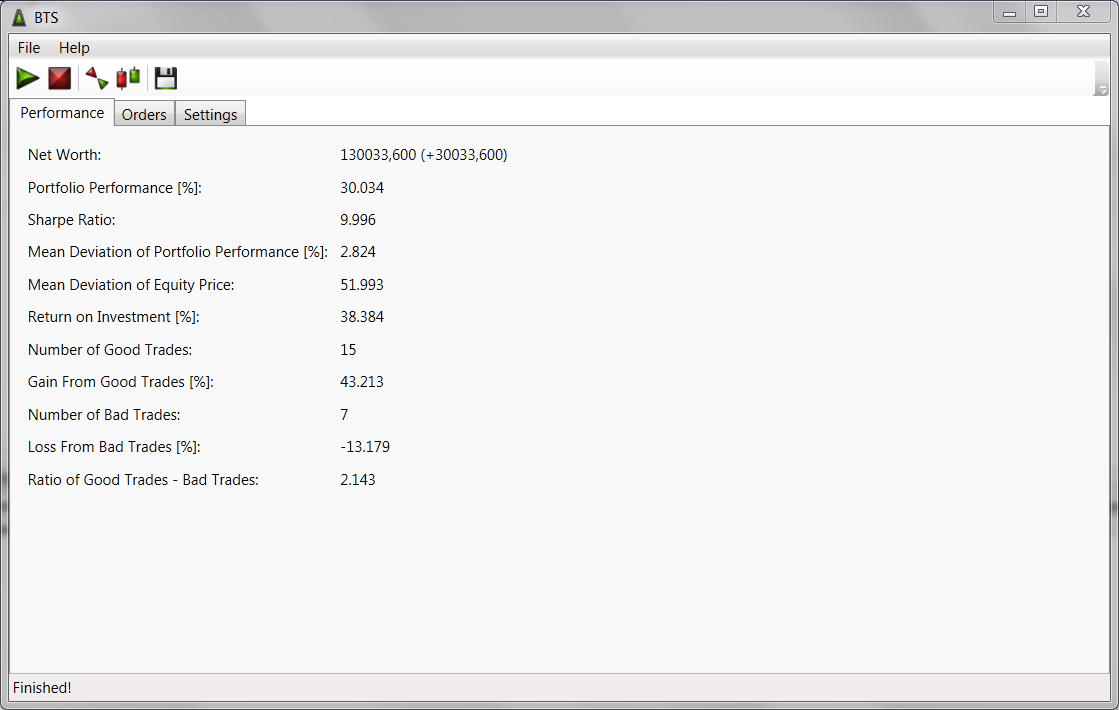
\includegraphics[width=1.00\textwidth]{graphics/ergebnis/bts_performance.png}
	\caption{Beispielhafte Darstellung allgemeiner Performancedaten nach einer Berechnung}
	\label{fig:bts_performance}
\end{figure}

Auf dem Orders-Tab erwartet den Benutzer bei derselben Konfiguration der Inhalt von Abbildung \ref{fig:bts_orders}.\\

\begin{figure}[!h]
	\centering
		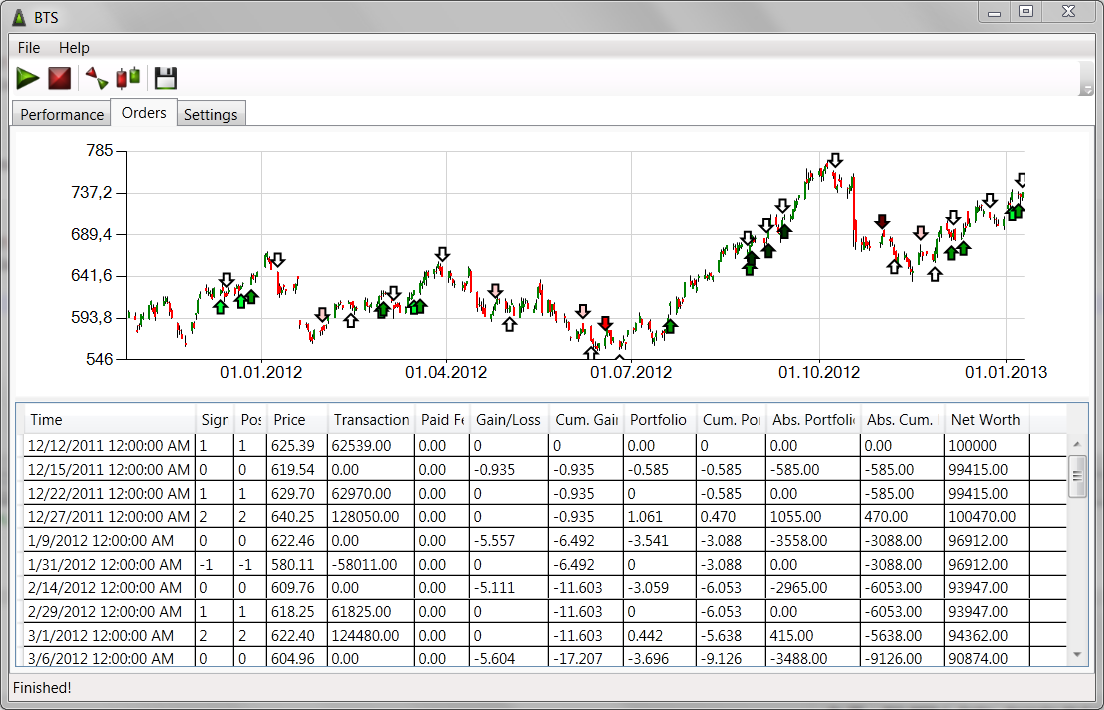
\includegraphics[width=0.90\textwidth]{graphics/ergebnis/bts_orders.png}
	\caption{Beispielhafte Darstellung des Orders-Tab nach einer Berechnung}
	\label{fig:bts_orders}
\end{figure}

Nun k�nnte man bspw. auf dem Settings-Tab unter "`Orders"' neue Einstellungen wie einen Price Premium (hierbei werden Aktien auch um einen geringf�gig h�heren/niedrigeren Betrag als den Ask/Bid gekauft/verkauft) und sowohl relative als auch absolute Transaktionsgeb�hren (Abgabe an den Broker f�r jede Transaktion) definieren. Diese haben teilweise drastische Auswirkungen f�r die Ergebnisse der Performance-Berechnung. So zum Beispiel senken relativ realit�tsnahe Einstellungen f�r die zuvor genannten Werte (siehe Abbildung \ref{fig:bts_fees}) bei der Nutzung derselben Daten und desselben Algorithmus die allgemeine Portfolio Performance von ca. 30\% auf ca. 15\% (siehe Abbildung \ref{fig:bts_performance_fees}).\\

\begin{figure}[!h]
	\centering
		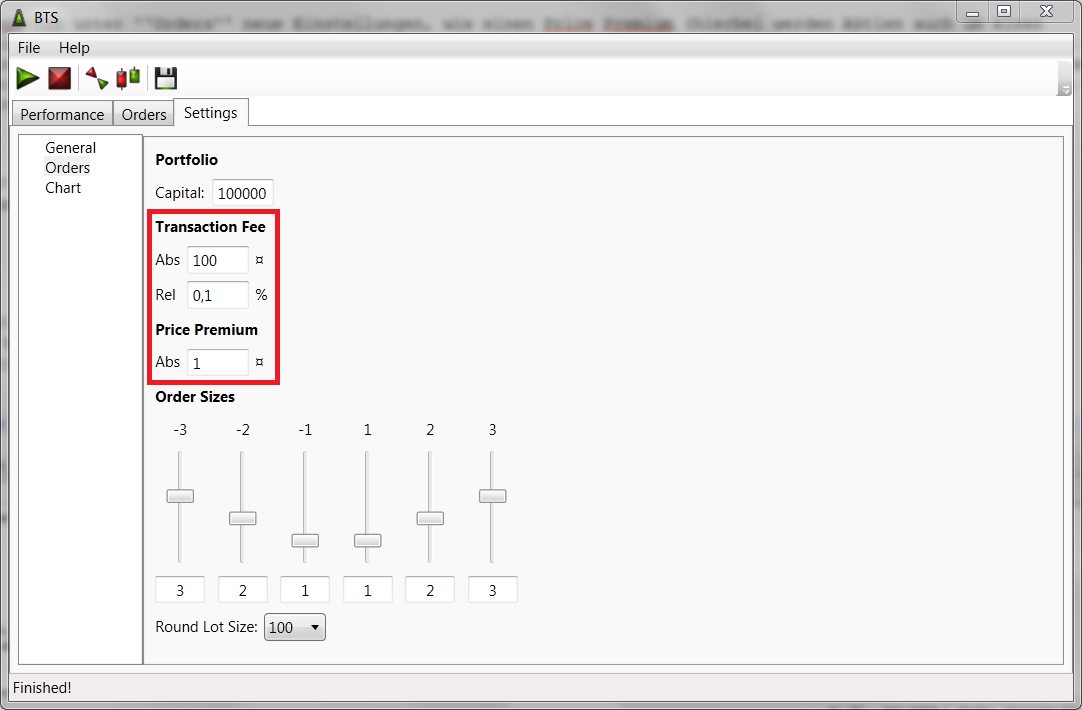
\includegraphics[width=0.90\textwidth]{graphics/ergebnis/bts_fees.png}
	\caption{Konfiguration von Transaktionsgeb�hren und einem Price Premium}
	\label{fig:bts_fees}
\end{figure}

\begin{figure}[!h]
	\centering
		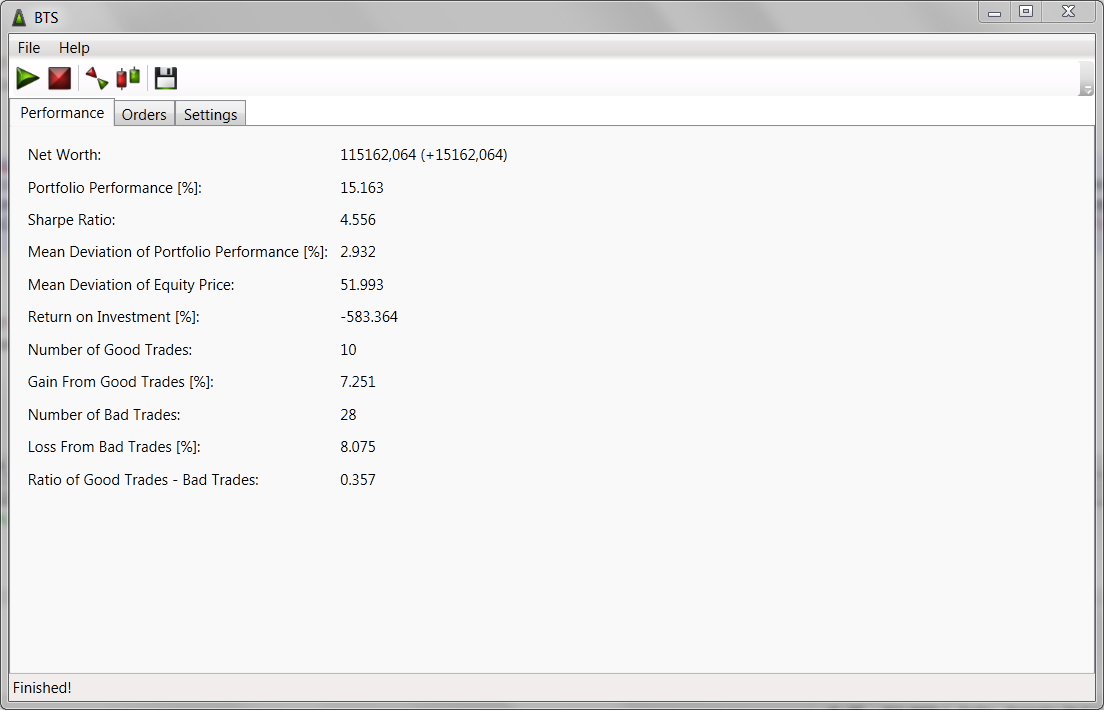
\includegraphics[width=0.90\textwidth]{graphics/ergebnis/bts_performance_fees.png}
	\caption{Performancedaten nach Ver�nderung der Einstellungen}
	\label{fig:bts_performance_fees}
\end{figure}

Weiters gibt es die M�glichkeit, die Anzahl an gekauften/verkauften Round Lots bei verschiedenen Signalen zu �ndern. Auch dies kann die Performance von Grund auf ver�ndern. Wenn man nun erneut mit denselben Einstellungen die Regler f�r alle verschiedenen Signale auf eine einheitliche Zahl (hier 2) stellt, werden bei jedem positiven Signal (1, 2 oder 3) gleich viele Round Lots gekauft und bei jedem negativen Signal (-1, -2 oder -3) gleich viele Round Lots verkauft. Zum Beispiel sinkt mit den Einstellungen aus Abbildung \ref{fig:bts_orderSizes} und allen anderen Einstellungen wie zuvor die allgemeine Portfolio Performance weiter auf nur ca. 8\%.\\

\begin{figure}[!h]
	\centering
		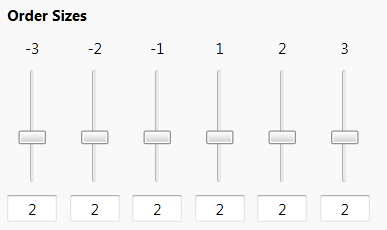
\includegraphics[width=0.50\textwidth]{graphics/ergebnis/bts_orderSizes.png}
	\caption{Konfiguration von gleichen Order Sizes f�r alle Signale}
	\label{fig:bts_orderSizes}
\end{figure}

Auf dem Orders-Tab kann man hier nun im unteren \inline{DataGrid} erkennen, dass die Einstellungen auch wirklich �bernommen wurden (siehe Abbildung \ref{fig:bts_order_feesNsizes}).\\

\begin{figure}[!h]
	\centering
		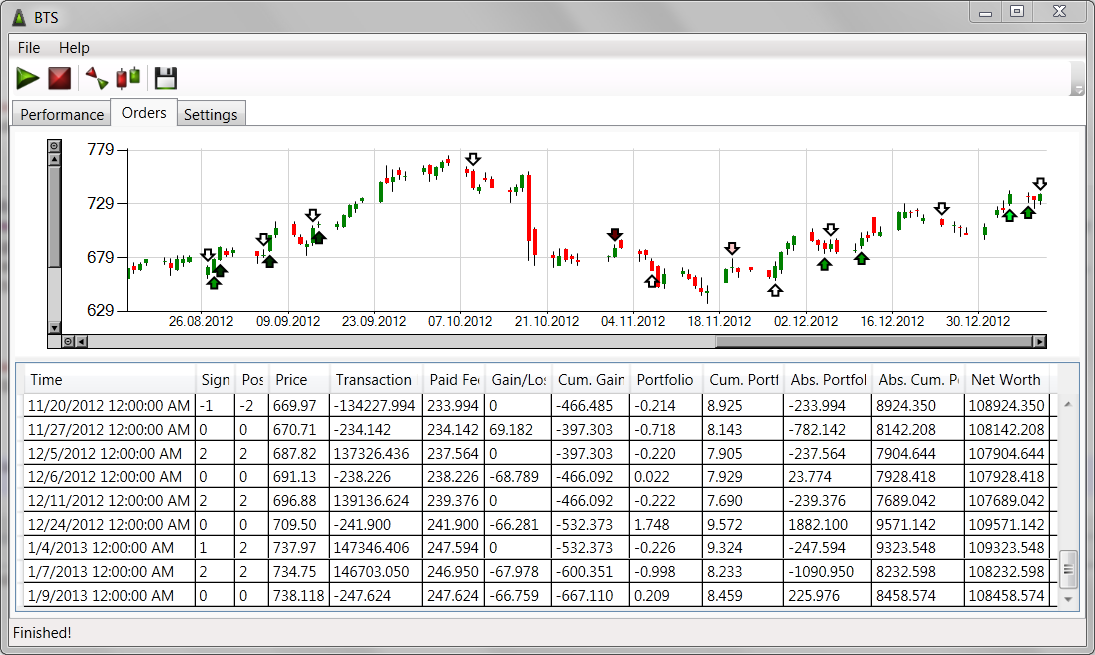
\includegraphics[width=0.90\textwidth]{graphics/ergebnis/bts_order_feesNsizes.png}
	\caption{Orders-Tab mit gleichen Order Sizes f�r alle Signale}
	\label{fig:bts_order_feesNsizes}
\end{figure}

Neben den performancetechnischen Daten k�nnen aber auch noch die rein optischen Indikatoren konfiguriert werden. Diese haben keinen Einfluss auf die eigentliche Berechnung, sie werden nur im Chart angezeigt und dienen als Erleichterung f�r den Benutzer. Es kann bspw. ein einfacher \gls{ma} mit der L�nge 10 und der Farbe Rot, ein \gls{wma} mit der L�nge 45 und der Farbe Gr�n, ein \gls{wma} mit der L�nge 90 und der Farbe Blau und ein \gls{macd} mit den L�ngen 10 und 90 und der Farbe Schwarz konfiguriert werden (siehe Abbildung \ref{fig:bts_indicators}) und sie werden genau so ins Chart eingezeichnet (siehe Abbildung \ref{fig:bts_chart_indicator}). F�r den \gls{macd} wird hierbei sogar eine eigene \inline{ChartArea} eingef�gt, da er um die Nulllinie fluktuiert.\\

\begin{figure}[!h]
	\centering
		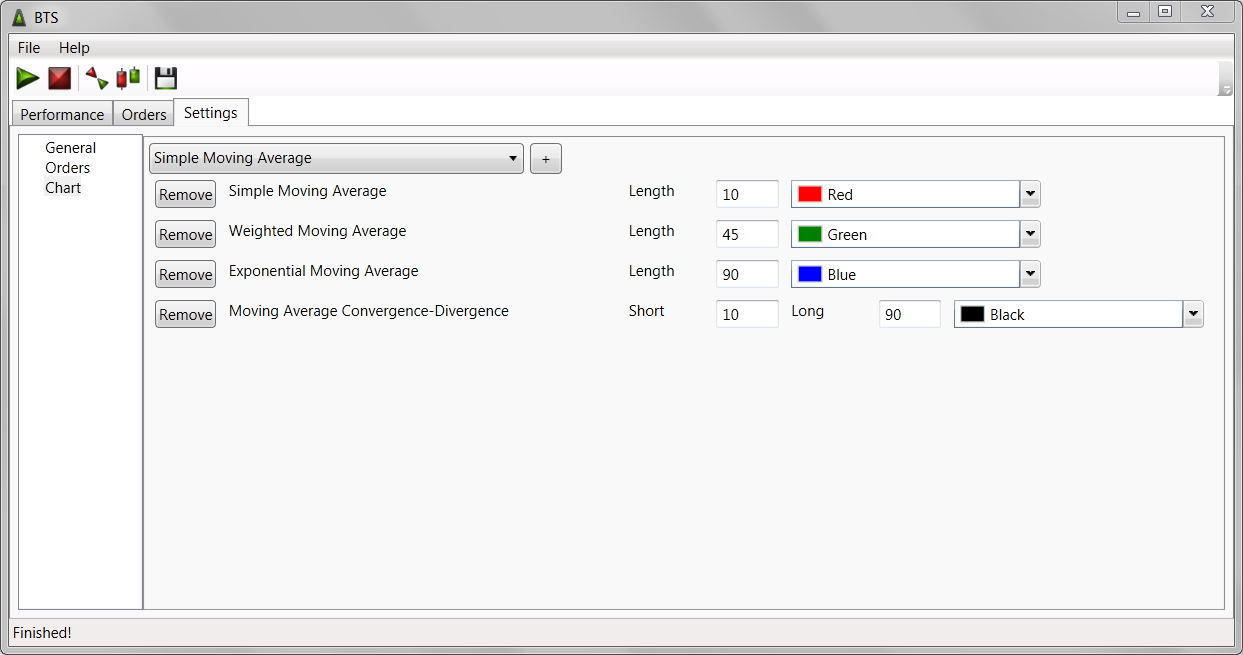
\includegraphics[width=0.90\textwidth]{graphics/ergebnis/bts_indicators.png}
	\caption{Konfiguration von verschiedenen Indikatoren zur Darstellung im Chart}
	\label{fig:bts_indicators}
\end{figure}

\begin{figure}[!h]
	\centering
		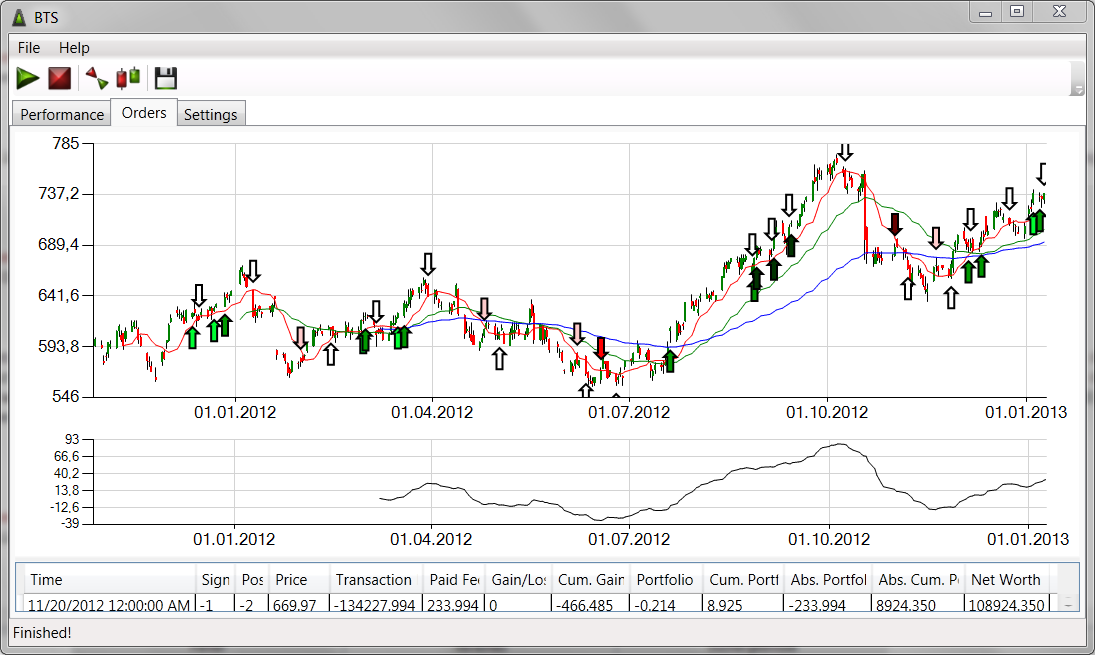
\includegraphics[width=0.90\textwidth]{graphics/ergebnis/bts_chart_indicator.png}
	\caption{Darstellung verschiedener Indikatoren}
	\label{fig:bts_chart_indicator}
\end{figure}

Bei allen Einstellungen, die im Laufe dieses Abschnitts get�tigt wurden, handelt es sich lediglich um Beispiele. Es k�nnen nat�rlich auch jegliche andere Zahlen als Price Premium oder Transaktionsgeb�hren gew�hlt werden. Au�erdem k�nnten andere Indikatoren, Order Sizes oder sogar ein anderes Startkapital gew�hlt werden. Hierbei hat der Benutzer die freie Wahl.